\chapter{Results}
\todo{Some intro to the chapter}

\clearpage
\section{Content Analysis Results}
From the retrospective reports we obtained several interesting results. We will go through each of them below starting with some key numbers and then move on to the results of the content analysis. Then we identify some trends observed while performing the content analysis. 

\subsection{Key Numbers}
In this section we will present some key numbers of the retrospective results and this numbers can also be seen in \autoref{table:key-numbers}.The retrospective reports spanned over a period of five years from August 2009 to November 2014. This is equal to 278 weeks and we are going to refer to week numbers from the first retrospective for the remainder of this report. 
\begin{table}[!h]
	\begin{center}
	\caption{Some key numbers from the retrospectives}
	\label{table:key-numbers}
	\makebox[\textwidth]{%
		\begin{tabular}{ l | p{0.5\textwidth}}
		\hline
		Key-value & Value  \\
		\hline
		Retrospective report period & 278 Weeks \\
		Number of total actions & 343 \\
		Number of unresolved actions & 65 \\
		Average actions per week & 1.23 \\
		Average unresolved action per week & 0.23 \\
		\hline
		\end{tabular}
	}
\end{center}
\end{table}
During the 278 weeks 77 retrospectives were held and and within these 343 actions was created, where 65 of these actions were still unresolved. This yields an average of 4.45 actions per retrospective and 0.84 unresolved per retrospective. This is equal to 1.23 actions per week, where one have 0.23 unresolved actions per week. 
In \autoref{figure:key-numbers} we can see the development of numbers of actions. We can see that the team has had a pretty steady amount of actions with no abnormal spikes or changes. The total amount of actions follows the average expected actions quite close and reveals the steady number of actions. The amount of active (or unresolved) actions also has a steady amount of total actions increasing at about the same rate as the total number of actions. 


\begin{sidewaysfigure}[!h]
	\centering
	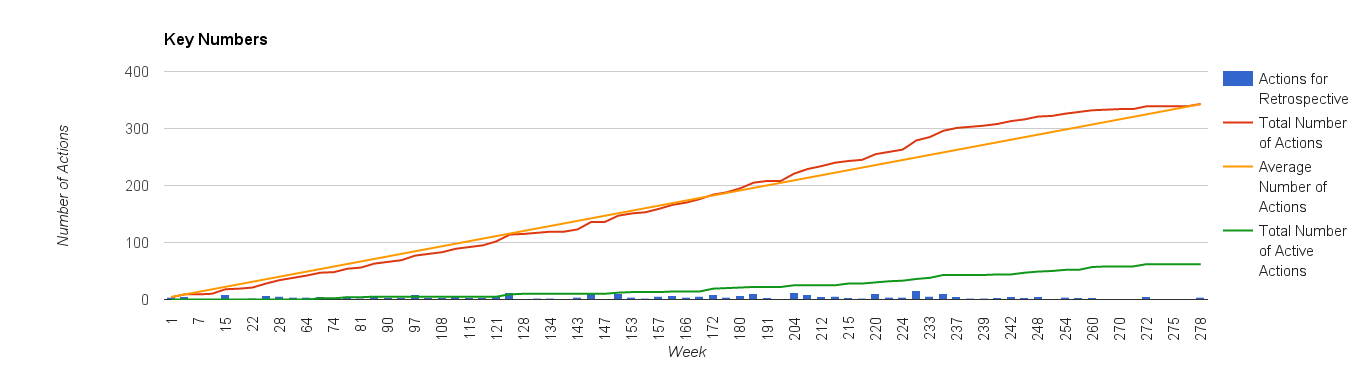
\includegraphics[width=\textwidth, keepaspectratio]{figures/key-numbers.png}
	\caption{A visual representation of some of the key numbers.}
	\label{figure:key-numbers}
\end{sidewaysfigure}
\clearpage	

\subsection{Analysis Results}
In this section we will present the results from our content analysis. We will present the results for each theme defined in \autoref{method:categories}. 

\subsubsection{Nature}
The content analysis revealed that most actions are created as a result of negative problems that has occurred during the development. 89.3\% of the actions were negative, while 5.5\% of the actions were positive and acknowledged good working practices that would be continued. 5.2\% of the actions we lacked the context to determine whether they were positive or negative. As for the distribution of the actions over each retrospective there was no abnormalities except week 97 where there was an unusual amount of positive actions. However while looking into this week we found nothing in particular that could be identified as cause for this spike. As can be seen in \autoref{figure:nature-pa} and \autoref{table:nature-results} the classification of the active actions pretty much mirrored the results from the total actions. 

\begin{table}[!h]
	\begin{center}
	\caption{Analysis results from the content analysis for the nature of the action.}
	\label{table:nature-results}
	\makebox[\textwidth]{%
		\begin{tabular}{| l | l | l | l | l |}
		\hline
		Category & \multicolumn{2}{|c|}{All Actions} & \multicolumn{2}{|c|}{Active Actions}  \\
		\cline{2-5}
		& Number & Percentage & Number & Percentage \\	
		\hline
		Positive & 19 & 5.5\% & 1 & 1.6\% \\
		Negative & 310 & 89.3\% & 57 & 90.5\% \\
		Undefined & 18 & 5.2\% & 5 & 7.9\% \\
		\hline
		\end{tabular}
	}
	\end{center}
\end{table}

\begin{figure}[!h]
	\centering
	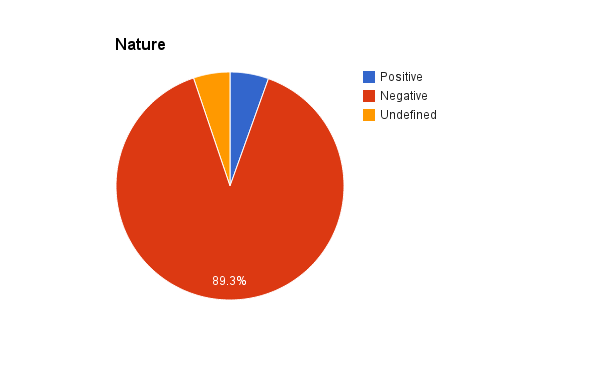
\includegraphics[width=\textwidth, keepaspectratio]{figures/nature-p.png}
	\caption{The negative, positive and undefined distribution of all the actions.}
	\label{figure:nature-p}
\end{figure}

\begin{figure}[!h]
	\centering
	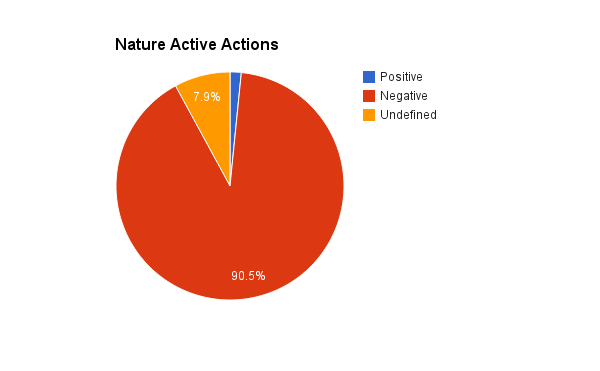
\includegraphics[width=\textwidth, keepaspectratio]{figures/nature-pa.png}
	\caption{The negative, positive and undefined distribution of the active actions.}
	\label{figure:nature-pa}
\end{figure}

\begin{sidewaysfigure}[!h]
	\centering
	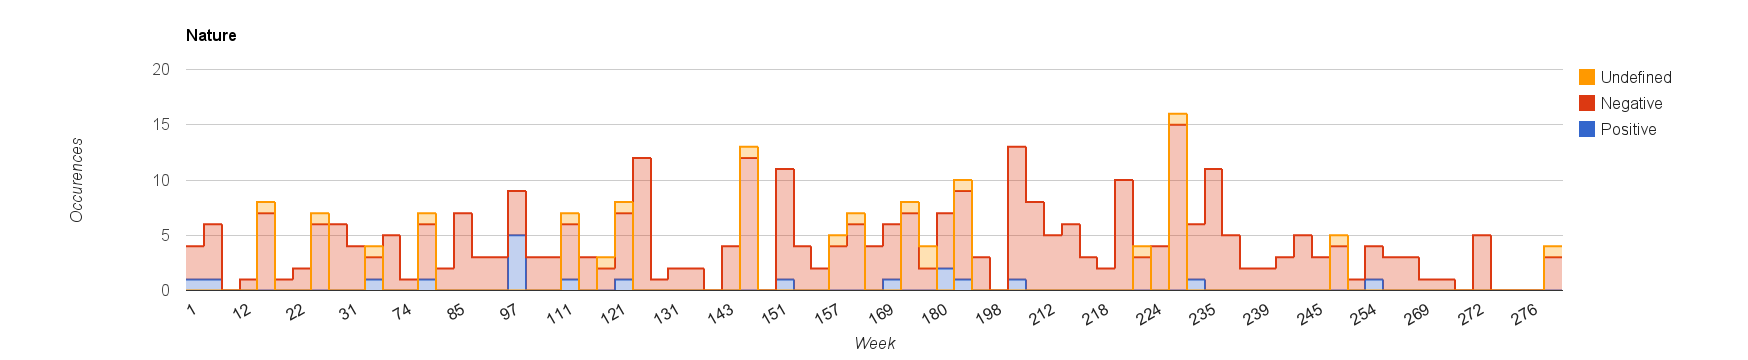
\includegraphics[width=\textwidth, keepaspectratio]{figures/nature-l.png}
	\caption{The distribution of negative, positive and undefined actions across the timespan}
	\label{figure:nature-l}
\end{sidewaysfigure}

\clearpage

\subsubsection{Context}
For the context of the actions analyzed mostly where process related ones. The process actions numbered in 228, which is equal to 58.6\% of all the actions. The Technical ones numbered as 157 which is 40.4\%, while only 4 actions were undefined which results in 1\% of the total actions. As for the distribution over the timespand analyzed there where no abnormalities as can be seen in \autoref{figure:context-l}. For the active actions the results become more equal as seen in \autoref{figure:context-pa}. However it is worth mentioning that the active actions are a sub-group of the total and thus this result is probably a skewed grouping. 

\begin{table}[!h]
	\begin{center}
	\caption{Analysis results from the content analysis for the context of the action.}
	\label{table:context-results}
	\makebox[\textwidth]{%
		\begin{tabular}{| l | l | l | l | l |}
		\hline
		Category & \multicolumn{2}{|c|}{All Actions} & \multicolumn{2}{|c|}{Active Actions}  \\
		\cline{2-5}
		& Number & Percentage & Number & Percentage \\	
		\hline
		Technical & 157 & 40.4\% & 37 & 52.1\% \\
		Process & 228 & 58.6\% & 34 & 47.9\% \\
		Undefined & 4 & 1\% & 0 & 0\% \\
		\hline
		\end{tabular}
	}
	\end{center}
\end{table}

\begin{figure}[!h]
	\centering
	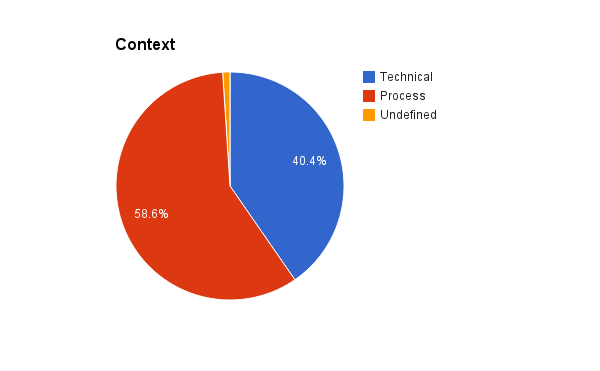
\includegraphics[width=\textwidth, keepaspectratio]{figures/context-p.png}
	\caption{The distribution of technical, process and undefined related actions.}
	\label{figure:context-p}
\end{figure}

\begin{figure}[!h]
	\centering
	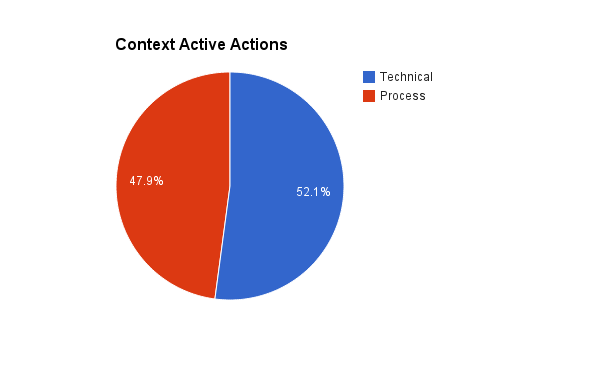
\includegraphics[width=\textwidth, keepaspectratio]{figures/context-pa.png}
	\caption{The distribution of technical, process and undefined related actions over.}
	\label{figure:context-pa}
\end{figure}

\begin{sidewaysfigure}[!h]
	\centering
	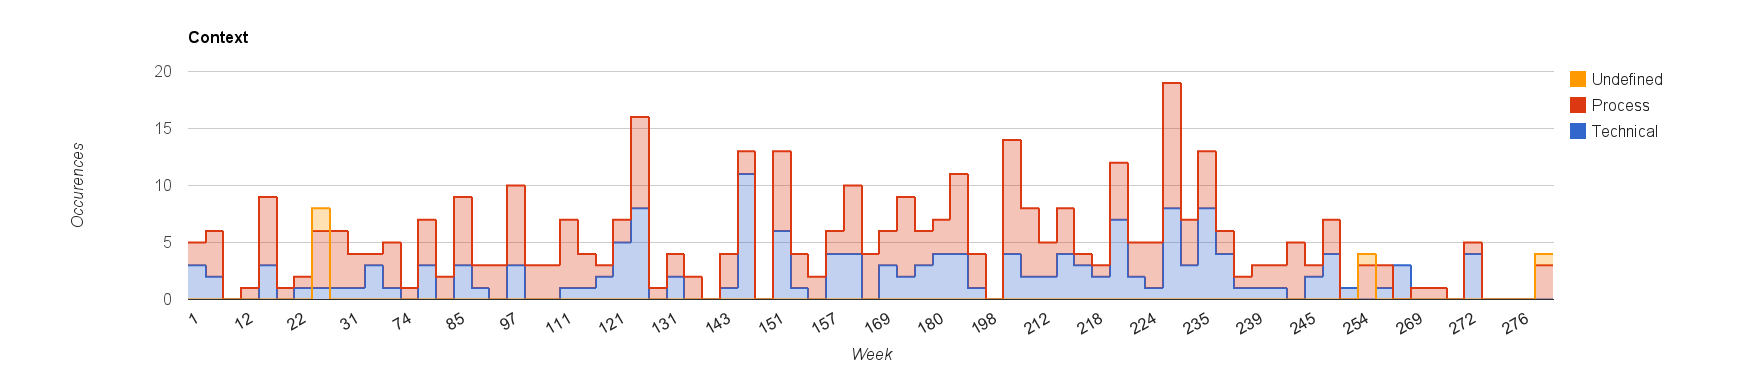
\includegraphics[width=\textwidth, keepaspectratio]{figures/context-l.png}
	\caption{The distribution of technical, process and undefined related actions across the timespan.}
	\label{figure:context-l}
\end{sidewaysfigure}

\clearpage

\subsubsection{Decision Making}
The decision making results showed that the operational decision occurred most in the actions as can be seen in \autoref{table:decision-making-results} and \autoref{figure:decision-p}. Operational decisions occurred in 53.2\% of the actions, while tactical was at 25.9\% and strategic was at 16.1\% of the actions. There only was four cases where we were not able to determine which kinds of decision making type it was. For the distribution over time, as shown in \autoref{figure:decision-l}, there was no emerging patterns and all the decision making types was evenly distributed. The active actions mirrored the total actions almost equal as can be seen in \autoref{figure:decision-p} and \autoref{figure:decision-pa}.

\begin{table}[!h]
	\begin{center}
	\caption{Analysis results from the content analysis for the decision making perspective of the action.}
	\label{table:decision-making-results}
	\makebox[\textwidth]{%
		\begin{tabular}{| l | l | l | l | l |}
		\hline
		Category & \multicolumn{2}{|c|}{All Actions} & \multicolumn{2}{|c|}{Active Actions}  \\
		\cline{2-5}
		& Number & Percentage & Number & Percentage \\	
		\hline
		Strategic & 55 & 16\% & 10 & 16.1\% \\
		Tactical & 89 & 25.9\% & 18 & 29\% \\
		Operational & 195 & 56.9\% & 33 & 53.2\% \\
		Undefined & 4 & 1.2\% & 1 & 1.6\% \\
		\hline
		\end{tabular}
	}
	\end{center}
\end{table}

\begin{figure}[!h]
	\centering
	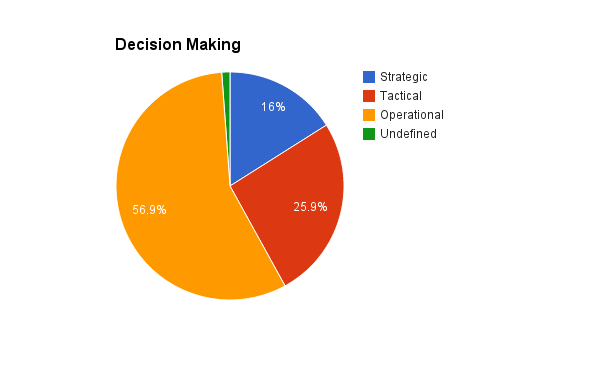
\includegraphics[width=\textwidth, keepaspectratio]{figures/decision-p.png}
	\caption{The distribution of different decision making decisions as they occurred over all the actions.}
	\label{figure:decision-p}
\end{figure}

\begin{figure}[!h]
	\centering
	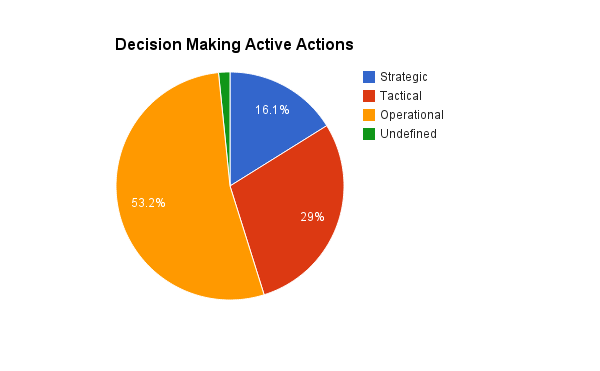
\includegraphics[width=\textwidth, keepaspectratio]{figures/decision-pa.png}
	\caption{The distribution of different decision making decisions as they occurred over the active actions.}
	\label{figure:decision-pa}
\end{figure}

\begin{sidewaysfigure}[!h]
	\centering
	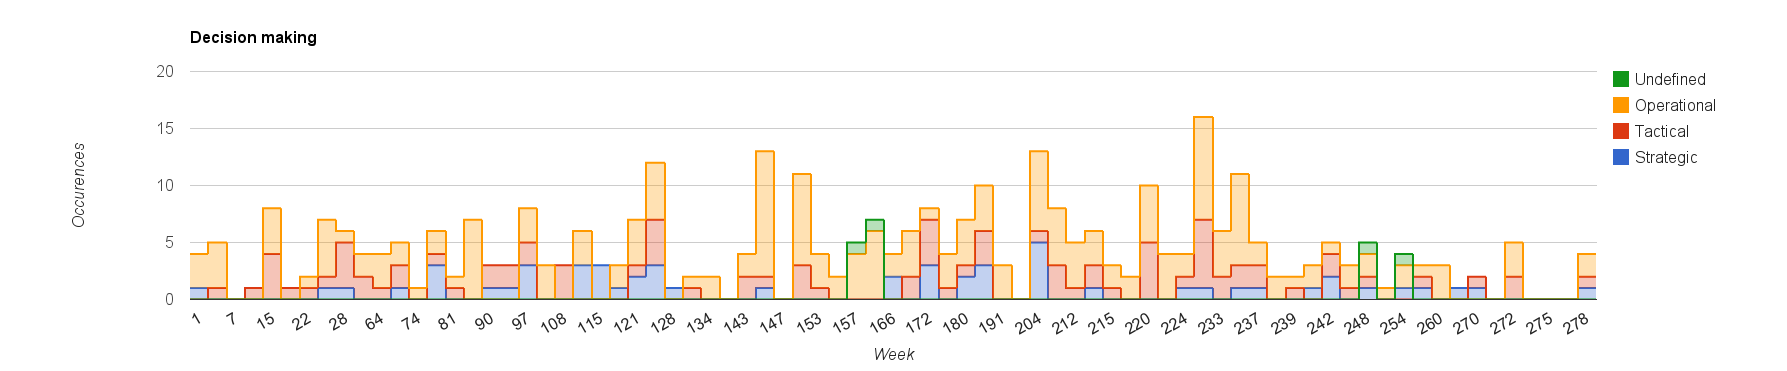
\includegraphics[width=\textwidth, keepaspectratio]{figures/decision-l.png}
	\caption{A timeline showing the distribution of the different decision making decisions for all the actions.}
	\label{figure:decision-l}
\end{sidewaysfigure}
\clearpage

\subsubsection{Organizational Learning}
In terms of organizational learning each action could be defined as single-loop, double-loop or undefined. The results yielded from the content analysis showed that single-loop was the most occurring type of organizational learning with 66.4\% of the actions. Double-loop had 27.2\% of actions, and the rest was undefined at 6.4\%. The distribution over the timespan, \autoref{figure:learning-l} of the analysis showed that the three categories was evenly distributed. The active actions was very similar to the total amount of actions and only had some small negligible variances as can be seen in \autoref{figure:learning-p} and \autoref{figure:learning-pa}.

\begin{table}[!h]
	\begin{center}
	\caption{Results from the content analysis regarding the organizational learning nature of the action.}
	\label{table:organizational-learning-results}
	\makebox[\textwidth]{%
		\begin{tabular}{| l | l | l | l | l |}
		\hline
		Category & \multicolumn{2}{|c|}{All Actions} & \multicolumn{2}{|c|}{Active Actions}  \\
		\cline{2-5}
		& Number & Percentage & Number & Percentage \\	
		\hline
		Single-loop & 227 & 66.4\% & 41 & 66.1\% \\
		Double-loop & 93 & 27.2\% & 16 & 25.8\% \\
		Undefined & 22 & 6.4\% & 5 & 8.1\% \\
		\hline
		\end{tabular}
	}
	\end{center}
\end{table}

\begin{figure}[!h]
	\centering
	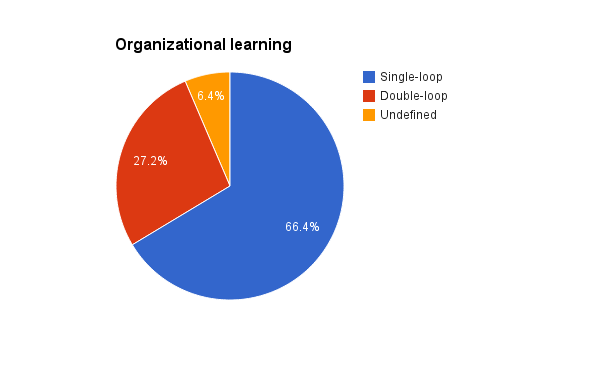
\includegraphics[width=\textwidth, keepaspectratio]{figures/learning-p.png}
	\caption{The distribution of single-loop, double-loop and undefined for all the actions.}
	\label{figure:learning-p}
\end{figure}

\begin{figure}[!h]
	\centering
	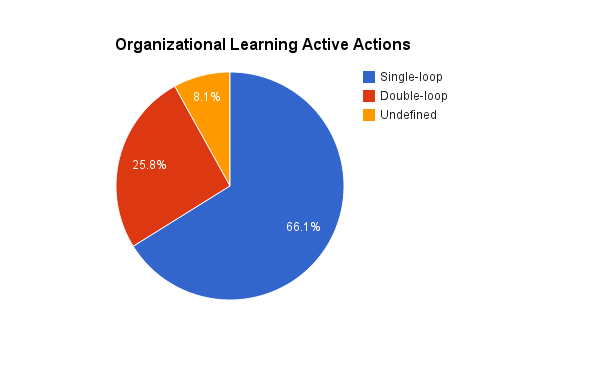
\includegraphics[width=\textwidth, keepaspectratio]{figures/learning-pa.png}
	\caption{The distribution of single-loop, double-loop and undefined for the active actions.}
	\label{figure:learning-pa}
\end{figure}

\begin{sidewaysfigure}[!h]
	\centering
	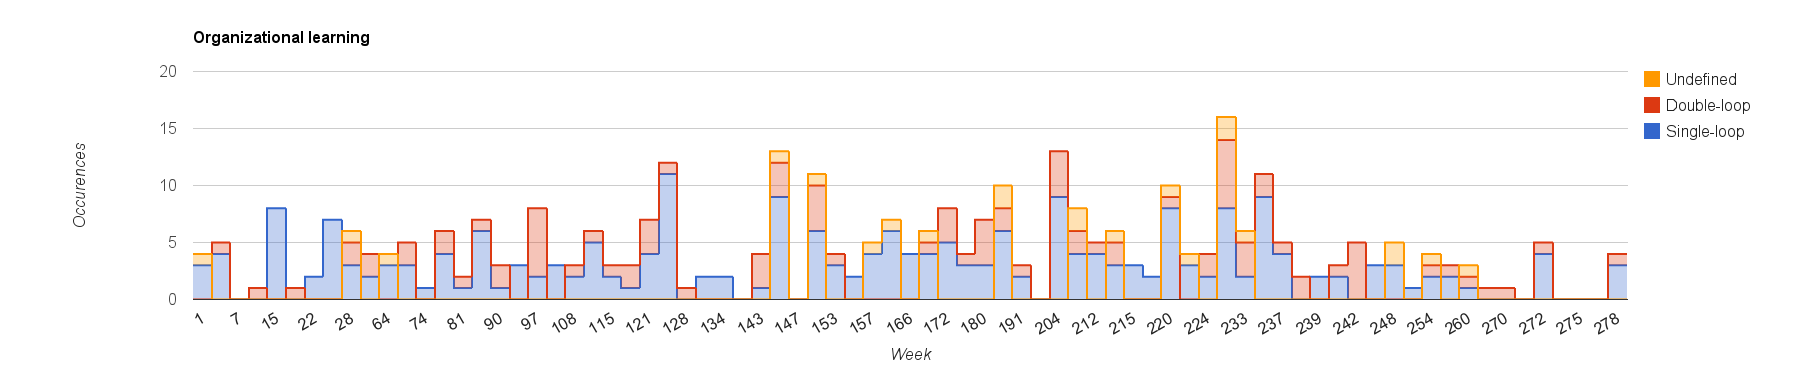
\includegraphics[width=\textwidth, keepaspectratio]{figures/learning-l.png}
	\caption{Timeline showing the distribution of learning loops for the total actions.}
	\label{figure:learning-l}
\end{sidewaysfigure}
\afterpage{\clearpage}

\subsubsection{Development Phase}
Planning, testing, development, and documentation were the four dominant phases in which an action were related according to our content analysis, as can be seen from \autoref{table:development-results} and \autoref{figure:development-p}. Planning being the biggest has a distribution value at 24.6\%. Second is the testing which 21.1\% of all the actions are related to. Development is related to 18.4\% and documentation is 13.2\%. Finally we have the remaining five categories Release, Build, Business Development, Bugfix and undefined which varies between 3.7-6.4 percent as can be seen in \autoref{table:development-results}. 
For the distribution of the different categories over time all of the categories are evenly distributed, in other words; No category is clustered to a specific period in time, but rather occurs evenly through the whole timespan. This can be seen in \autoref{figure:development-l}.
As have been the cases with the other themes the sub-group of the active actions mirrors the total actions with only minor variances as can be seen in \autoref{figure:development-pa} and \autoref{figure:development-p}.

\begin{table}[!h]
	\begin{center}
	\caption{Results from the content analysis in which development phase the action regards.}
	\label{table:development-results}
	\makebox[\textwidth]{%
		\begin{tabular}{| l | l | l | l | l |}
		\hline
		Category & \multicolumn{2}{|c|}{All Actions} & \multicolumn{2}{|c|}{Active Actions}  \\
		\cline{2-5}
		& Number & Percentage & Number & Percentage \\	
		\hline
		Development & 89 & 18.4\% & 11 & 13.1\% \\
		Testing & 102 & 21.1\% & 18 & 21.4\% \\
		Documentation & 64 & 13.2\% & 16 & 19\% \\
		Release & 18 & 3.7\% & 4 & 4.8\% \\
		Build & 23 & 4.8\% & 6 & 7.1\% \\
		Business Development & 18 & 3.7\% & 5 & 6\% \\
		Planning & 119 & 24.6\% & 19 & 22.6\% \\
		Bugfix & 20 & 4.1\% & 2 & 2.4\% \\
		Undefined & 31 & 6.4\% & 3 & 3.6\% \\
		\hline
		\end{tabular}
	}
	\end{center}
\end{table}

\begin{figure}[!h]
	\centering
	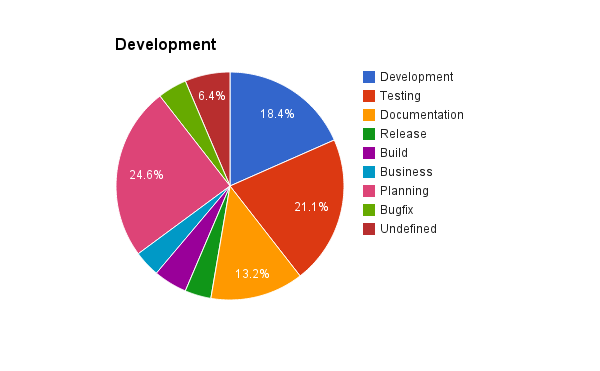
\includegraphics[width=\textwidth, keepaspectratio]{figures/development-p.png}
	\caption{The distribution of the different development phases for all the actions.}
	\label{figure:development-p}
\end{figure}

\begin{figure}[!h]
	\centering
	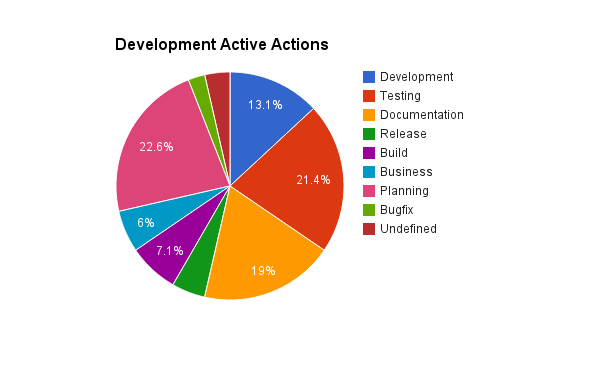
\includegraphics[width=\textwidth, keepaspectratio]{figures/development-pa.png}
	\caption{The distribution of the different development phases for the active actions.}
	\label{figure:development-pa}
\end{figure}

\begin{sidewaysfigure}[!h]
	\centering
	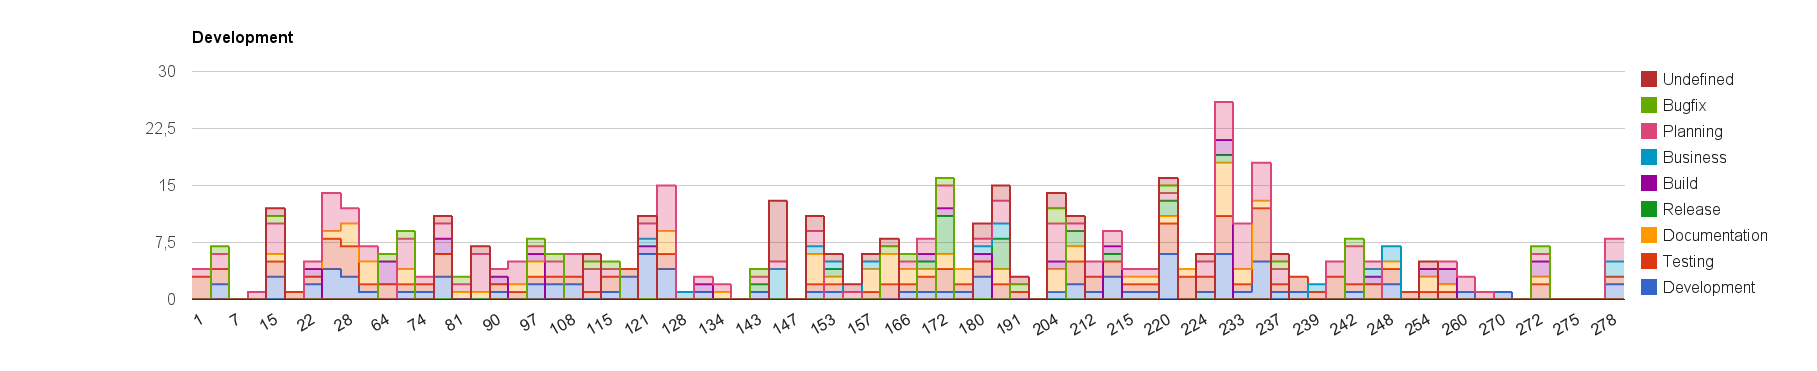
\includegraphics[width=\textwidth, keepaspectratio]{figures/development-l.png}
	\caption{Timeline showing the distribution of the different development phases over time.}
	\label{figure:development-l}
\end{sidewaysfigure}
\clearpage

\subsubsection{Collaboration}
Our results from the content analysis in terms of collaboration showed that 45.3\% of the actions were undefinable in terms of the analysis categorizations we had created. From the actions that were definable Communication was the biggest with 35.2\%. The second was external relations at 11.5\% and third competence at 6.9\%. Finally leadership was the smallest at 1.1\% of the total actions. The statistics can be seen in \autoref{table:collaboration-results} and \autoref{figure:management-p}. 
For the distribution of the different categories over time, \autoref{figure-management-l}, most of the categories was evenly spread across the whole timespan. the only exception to this is week 146 where there is a clear spike of external relations. This spike was a result of the team attending a network meeting in which they did a retrospective to better prepare them for the next network meeting. This anomaly will be disregarded further in the report. 
The active actions, \autoref{figure:management-pa}, shows that the three categories communication, competence and external relations evens out while leadership and undefined remains nearly the same only some small variances. However it is worth mentioning that the active actions are a sub-group of the total and thus this result is probably a skewed grouping. 

\begin{table}[!h]
	\begin{center}
	\caption{Results from the content analysis regarding the collaboration influences of an action.}
	\label{table:collaboration-results}
	\makebox[\textwidth]{%
		\begin{tabular}{| l | l | l | l | l |}
		\hline
		Category & \multicolumn{2}{|c|}{All Actions} & \multicolumn{2}{|c|}{Active Actions}  \\
		\cline{2-5}
		& Number & Percentage & Number & Percentage \\	
		\hline
		Communication & 128 & 35.2\% & 14 & 20.9\% \\
		Leadership & 4 & 1.1\% & 1 & 1.5\% \\
		Competence & 25 & 6.9\% & 1 & 11.9\% \\
		External relations & 42 & 11.5\% & 11 & 16.4\% \\
		Undefined & 185 & 45.3\% & 33 & 48.3\% \\
		\hline
		\end{tabular}
	}
	\end{center}
\end{table}

\begin{figure}[!h]
	\centering
	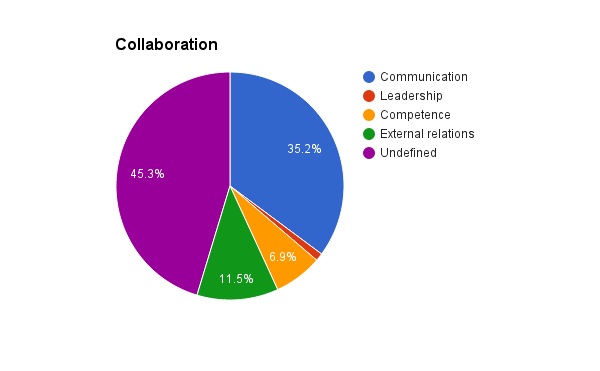
\includegraphics[width=\textwidth, keepaspectratio]{figures/management-p.png}
	\caption{The distribution of different collaboration categories for all the actions.}
	\label{figure:learning-p}
\end{figure}

\begin{figure}[!h]
	\centering
	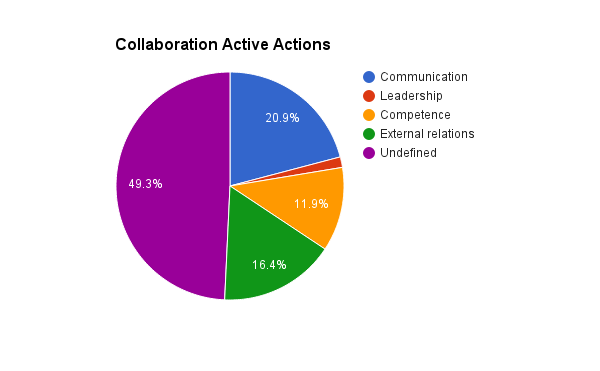
\includegraphics[width=\textwidth, keepaspectratio]{figures/management-pa.png}
	\caption{The distribution of different collaboration categories for the active actions.}
	\label{figure:learning-pa}
\end{figure}

\begin{sidewaysfigure}[!h]
	\centering
	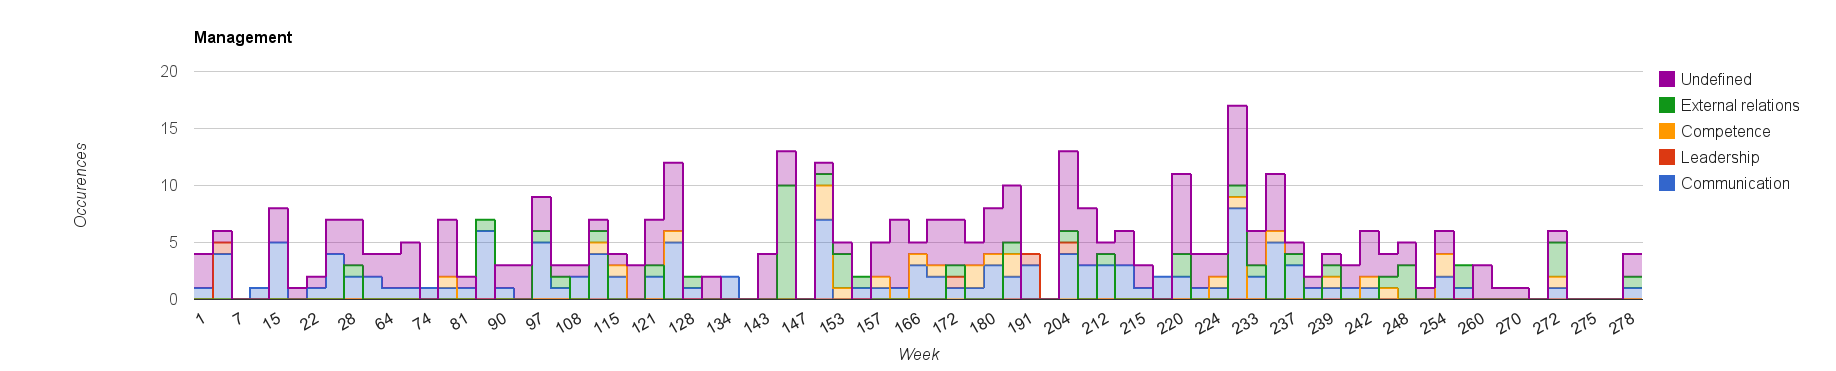
\includegraphics[width=\textwidth, keepaspectratio]{figures/management-l.png}
	\caption{Timeline showing the distribution of the different collaboration categories over time.}
	\label{figure:learning-l}
\end{sidewaysfigure}
\afterpage{\clearpage}

\subsection{Trends}
While conducting our content analysis of all the retrospective actions we uncovered some trends. By trend we mean actions that are related to the same issue/theme. We identified three trends being; Bugfix, Scenario Template and Developer-Tester Communication. We'll go through each of these in the following sub-sections.

\subsubsection{Bugfix}
The first trend we recognized performing our content analysis was bugfixing. Developing computer systems is sure to create bugs and fixing them then becomes a natural part of developing software. In total we found 20 actions that was related to bugfixing. Of these two were purely technical actions, five were technical and process related and the remaining 13 action were purely process related. Of the 20 actions nine were related to communication between team members. In \autoref{figure:bugfix} one can see that the total amount of bugfixing actions has increased steadily throughout the timespan. 

\begin{figure}[!h]
	\centering
	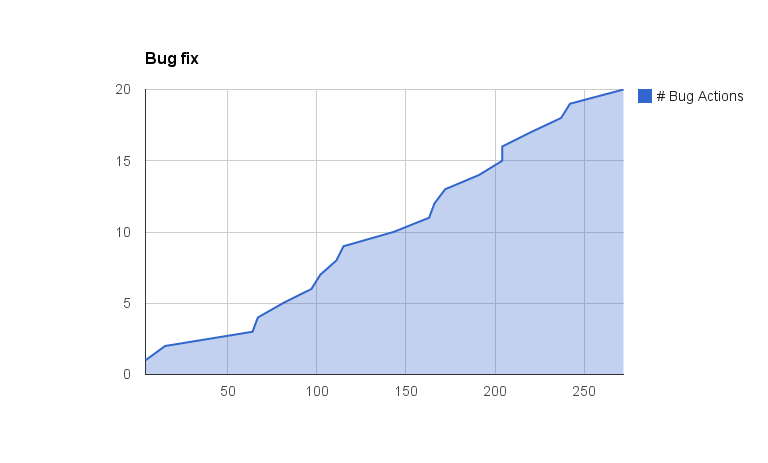
\includegraphics[width=\textwidth, keepaspectratio]{figures/bugfix.png}
	\caption{The total amount of bugfix actions over time.}
	\label{figure:bugfix}
\end{figure}

\subsubsection{Scenario Template}
For the second trend we discovered was in relation to a worktool called scenario template that team used to help specify requirements, create user stories and etc. In total we found 25 actions that were related to the scenario template. Of these 25 actions four of the actions were technical and process related, six were purely technical adjustments of the tool and 16 of the actions were process oriented on how the scenario template should be used. 18 of the actions were single-loop, only changing the effects which the scenario template provided. There were also six double-loop actions acknowledging root-cause issues with using the scenario-template and changes to reflect them. 
In \autoref{figure:scenario-template} the total amount of scenario template actions are shown over the 272 week long timespan. One can see that until week 163 the team has a slow increase in the number of scenario template actions. After week 163 however. a huge increase in number of scenario template actions occur. This continues until week 235, with a little slow period between week 180 and 205. At week 235 the team planned a meeting to go through the complete scenario template and after week 235 there are no more actions related to the scenario template. 

\begin{figure}[!h]
	\centering
	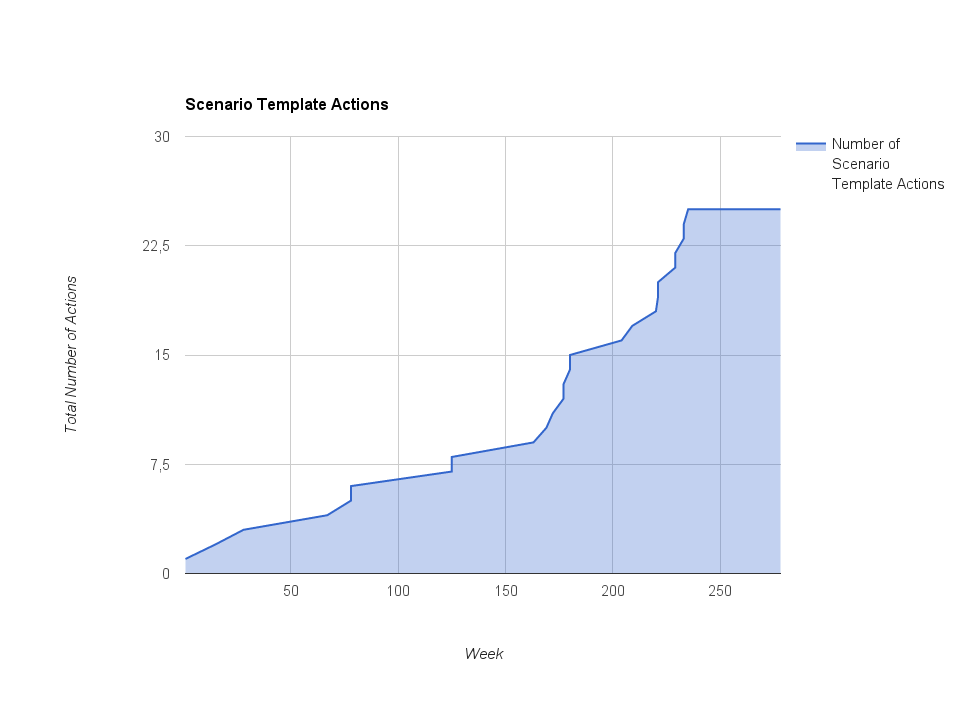
\includegraphics[width=\textwidth, keepaspectratio]{figures/Scenario-tpl.png}
	\caption{The total amount of scenario template actions over time.}
	\label{figure:scenario-template}
\end{figure}

\subsubsection{Developer-Tester Communication}
The final trend we observed during our content analysis was the communication between developers and testers. In total 25 actions were related to this. Of these 24 were process oriented and all the actions occurred from issues with a negative nature. 
\autoref{figure:dev-test-com} shows the distribution of the 25 actions over the 272 week long timespan. It can be seen that for the first 209 weeks that the amount of actions increase slowly with only two to seven actions every 50th week. After week 209 however we see a dramatic increase in the amount of actions, before it completely stops in week 238. We were not able to find any possible reasons for this sudden stop from reading through the reports. However as can be seen from \autoref{figure:dev-test-com} there has been periods between actions as long as 45 weeks so it is possible that this stop can be such a break.  

\begin{figure}[!h]
	\centering
	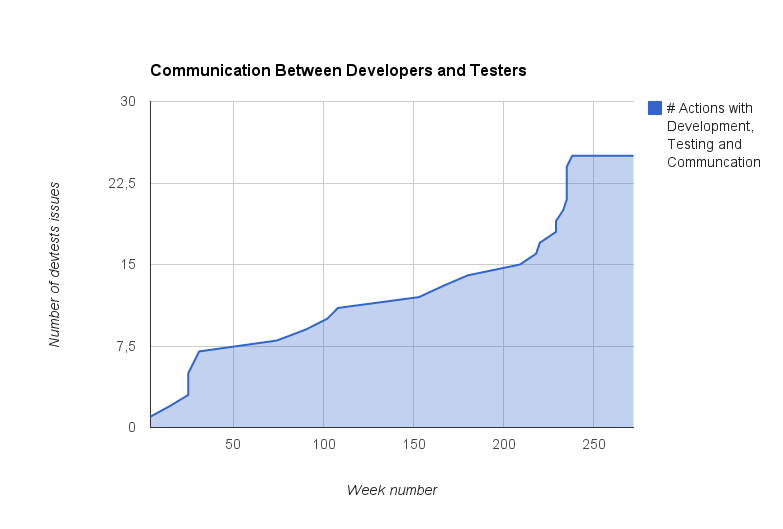
\includegraphics[width=\textwidth, keepaspectratio]{figures/devtestcom.png}
	\caption{The total amount of developer-tester communication related actions shown over time.}
	\label{figure:dev-test-com}
\end{figure}

\afterpage{\clearpage}

